\section{Interpreting the correlation coefficient, $r$}

\begin{tcolorbox}[center,width=5.5in]
    \small
    To \gap{interpret} \gap{$r$},
    say how well (or poorly) you think the variables in the problem
    are correlated to each other.
    \begin{itemize}[nosep]
        \item Find the location of $r$ on this diagram.\\
        {
            \centering
            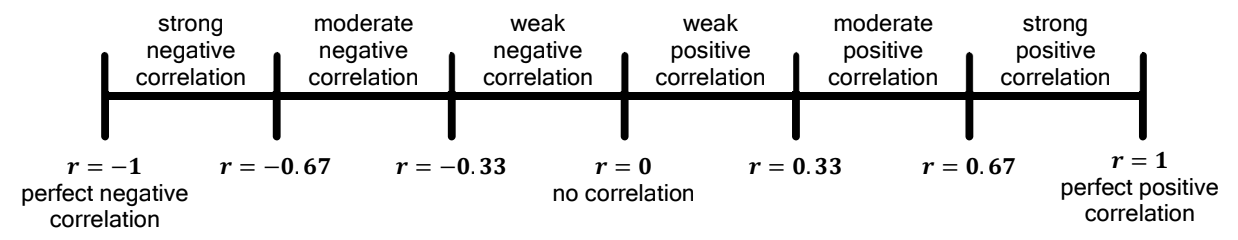
\includegraphics[height=0.8in]{correlation-strengths.png}
        }
        \item Write your answer as\\
        {
            \small\itshape 
            The value of $r$ suggests that 
            \gap{x variable} and \gap{y variable}
            are 
            \underline{\hspace{1.5in}} correlated.
        }
    \end{itemize}
\end{tcolorbox}

\myProblems[Interpret $\bm{r}$ for the given variables.]
{
    $x$: foot length, $y$: height, \hfill $\bm{r}=0.82$
}
{
    $x$: year, $y$: finish time, \hfill $\bm{r}=-0.56$
}
{1in}